\chapter{The straw tracker}\label{chaptertrk}

\textit{This Chapter provides a brief introduction on the working principles 
of a drift tube and then a  detailed description of the Mu2e straw tracker. 
This includes a description of the tracker mechanical structures 
(straw, panels, planes and stations) and the Front-End and DAQ electronics. 
Most of the discussion is based on \cite{kola} and \cite{bobbb}.}

\section{Drift Tubes}
Gas detectors are capable of measuring charged particle coordinates. 
They provide spatial resolution which could be as good as 50 $\mu$m
and high detection efficiency at a low cost \cite{kola}. 
There are many different gas ionizazion detectors, one of which is the drift tube.
The basic configuration of a drift tube is shown in Figure \ref{fig:drifttube}.
A hollow cylindrical conducting tube is grounded and serves as the cathode.
The tube is filled with a combination of a noble gas, often Argon, and a quench gas. 
A thin sensing wire is positioned along the cylindrical cathode axis. 
The wire, called anode, receives a high voltage. 

\begin{figure}[!h]
    \centering
    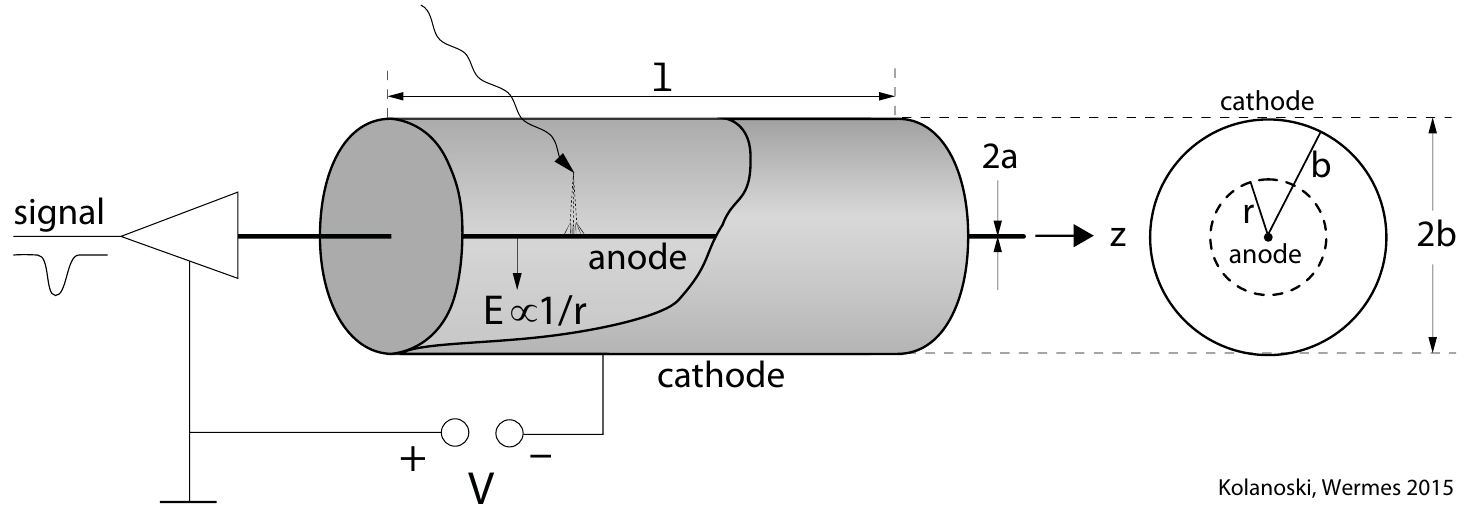
\includegraphics[width =0.8\textwidth]{figures/png/Screenshot_20240324_232621.png}
    \caption[Schematic view of a drift tube.]{Schematic view of a drift tube \cite{kola}.}
    \label{fig:drifttube}
    \end{figure}
Assuming an anode radius $a$, a cathode radius $b$ and using Gauss theorem, the electric field is:
\begin{equation}\label{avalanche}
    E(r)=\frac{1}{r}\frac{\lambda}{2\pi \epsilon}=\frac{1}{r}\frac{V}{ \text{ln}(b/a)} \qquad (a<r<b)
\end{equation}
Where $\lambda$ is linear charge density on the wire and $\epsilon$ is the dielectric constant of the gas.
Lower diameter wires are typically preferred in drift tubes.
A higher electric field near the wire increases the amplification factor 
of the drift tube at the same voltage. Additionally, smaller diameter of a signal wires 
improves the spatial resolution \cite{kola}. 
\subsection{Gas Ionization}
There are two types of interactions that can deposit energy as particles traverse the gas volume: ionization and excitation.
Collisions between a charged particle $C$ and an atom $A$ can result in the ejection of one or more electrons: 
$A \ C \rightarrow A^+ e^- C$, or $A \ C \rightarrow A^{++} e^- e^- C$, if more than one electron is released.
This process is called primary ionisation. The mean energy loss per path length can be determined using the Bethe-Bloch formula.
A noble gas atom $A$ can turn also into an excited state $A^*$ through the interaction $A \ C \rightarrow A^* C$. 
In case of a compound gas (A+B), if the excitation energy of $A^*$ is higher 
than the ionization potential of $B$, the quencher, the
Penning Effect can produce ionization through $A^*B \rightarrow A B^+ e^-$.
In addition, noble gases can
also form molecular ions through processes such as $A^* A \rightarrow A_{2}^{*} \rightarrow A^+_2 e^-$.
A secondary ionisation can occur through these processes or through electrons that have sufficient energy for generating more ions.
To compute the average number of electron-ion pairs produced by the initial particle,
divide its total energy loss by the average energy required to make an electron-ion pair.
Due to the energy lost during excitation, this average 
does not match the gas ionisation potential. Measurements showed an average of one electron-ion pair every 
30 eV, with variations depending on gas composition and starting particle. Except for very slow particles, 
this value remains constant regardless of their initial energy.
Without an electric field, electrons and ions created during ionisations spread uniformly. 
Collisions cause them to lose energy and eventually reach thermal equilibrium with the surrounding gas. 
They eventually recombine. An electron maximal range during ionisation is correlated with its initial kinetic 
energy. In a normal temperature and pressure gas, a 10 keV electron may be stopped in approximately 1 mm. 
Ionisation electrons often have lower kinetic energy,
leading to a shorter range.
\subsection{Drift of Ions and Electrons}
An electric field accelerates free electrons and ions towards the anode and cathode 
along the field lines. As these particles accelerate, they scatter on other particles in the gas, 
losing energy. The directions of motion are randomised, and maximum speeds are set. As a result, 
these particles move uniformly along the electric field. This is referred to as the drift velocity of the 
charge. It is superimposed with the thermal motion.
Drift velocities for ions and electrons varies based on several parameters. Ions have a larger mass 
than electrons and their masses are comparable to those of gas molecules. During collisions, gas 
molecules absorb a significant portion of the energy gained from ions during acceleration. In a drift 
tube detector just a little amount of electric field energy enters the energy associated with ion motion, 
making it comparable to the initial thermal energy before acceleration. 
The ion drift velocity $v_i$ is proportional to the reduced electric field $E/N$ where N is the number density of the gas 
and it is typically $\mathcal{O}(10^3)$ cm/s, 
except in the region near to the anode wire where a stronger 
electric field is present. The ion thermal velocity is typically $\mathcal{O}(10^4)$ cm/s at room temperature.
On the opposite, only a small fraction of the energy is released during elastic collision from electrons, 
so they acquire more energy from the electric field than their thermal energy.
Many different factors impact electron drift velocity. Some gas molecules, such as H$_2$O or CO$_2$, 
can interact with electrons to produce negative ions due to their great electron affinity. In rare situations, 
electrons gather enough energy to exceed gas molecule excitation threshold, resulting in inelastic collisions. 
Electron drift velocity is a complex function of electric field intensity due to several variables influencing 
electron collisions across a large energy range. Figure \ref{fig:drift} shows the electron drift
velocity at different electric field strengths in argon-carbon dioxide mixtures (Ar-CO$_2$) of different
proportions \cite{ZHAO1994485}.
\begin{figure}[!h]
    \centering
    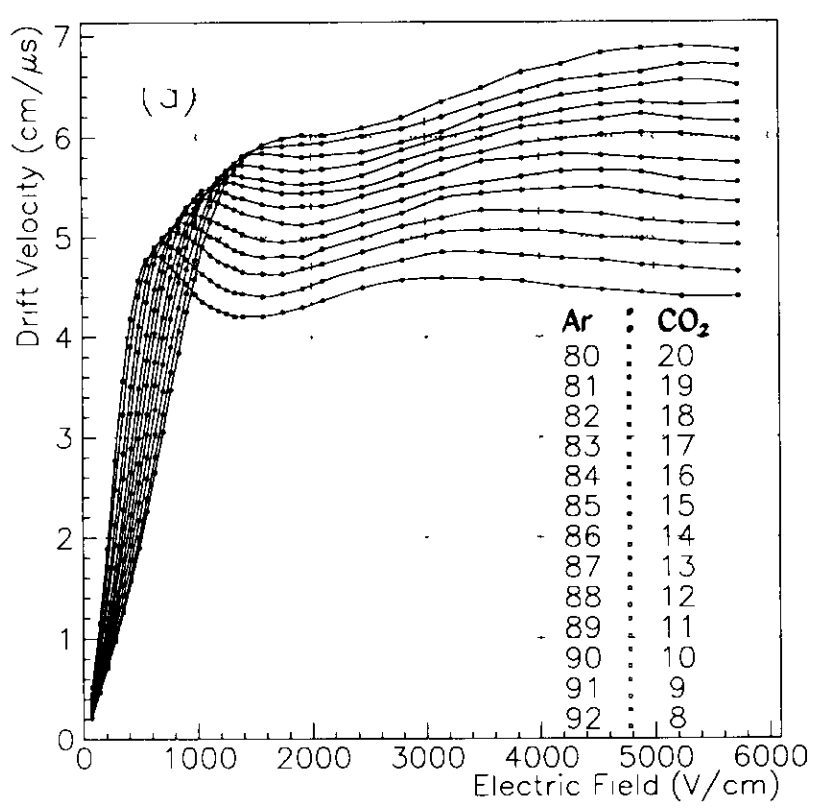
\includegraphics[width =0.7\textwidth]{figures/png/Screenshot_20240330_102206.png}
    \caption[Electron drift velocity versus electric field in Ar:CO$_2$ mixtures.]{Electron drift velocity versus electric field in Ar:CO$_2$ mixtures of different proportions \cite{ZHAO1994485}. 
    80\%:20\% Ar:CO$_2$ mixture is the gas used in the Mu2e tracker.}
    \label{fig:drift}
\end{figure}
Electron drift velocities in drift tubes are typically $\mathcal{O}(10^6)$ cm/s. 
This is significantly higher than ion drift velocities and comparable to electron
thermal velocity under the same conditions. 
The radial coordinate of an ionisation can be computed using the electron drift velocity and time.
Since drifting electrons and ions are scattered on gas molecules, they also diffuse along their trajectory. 
Electrons diffuse significantly quicker than ions because of their high velocity. Electron diffusion limits 
the intrinsic resolution of drift tubes used to measure incoming particle coordinates. CO$_2$ has internal 
degrees of freedom at low collision energies, preventing electron energies from exceeding thermal energy until 
field strengths above about 2 kV/cm. This improves intrinsic spatial resolution.
\subsection{Avalanche Multiplication}
Electrons can ionise when they face a high electric field near the anode wire. 
The released secondary electrons form tertiary electrons, and so on.
The number of free electrons rapidly increases, 
resulting in an avalanche. In a drift tubes, where the electron mean free path is about the order of $\mu$m, 
an avalanche develops when the electric field approaches $\mathcal{O}(10)$ kV/cm.
According to Equation \ref{avalanche}, using $a \sim \mathcal{O}(10^{-3})$ cm, $b \sim \mathcal{O}(1)$ cm and
a normal voltage of 1-2 kV, the avalanches can occur within $\mathcal{O}(100) \ \mu$m from the anode wire. 
Electrons from the avalanche are collected on the anode wire within 1 ns, while positively charged ions move towards the cathode.
Drifting ions mostly generate signals in electrodes via induction. Figure \ref{fig:avalanche} shows the model of an ionisation avalanche.
\begin{figure}[!h]
    \centering
    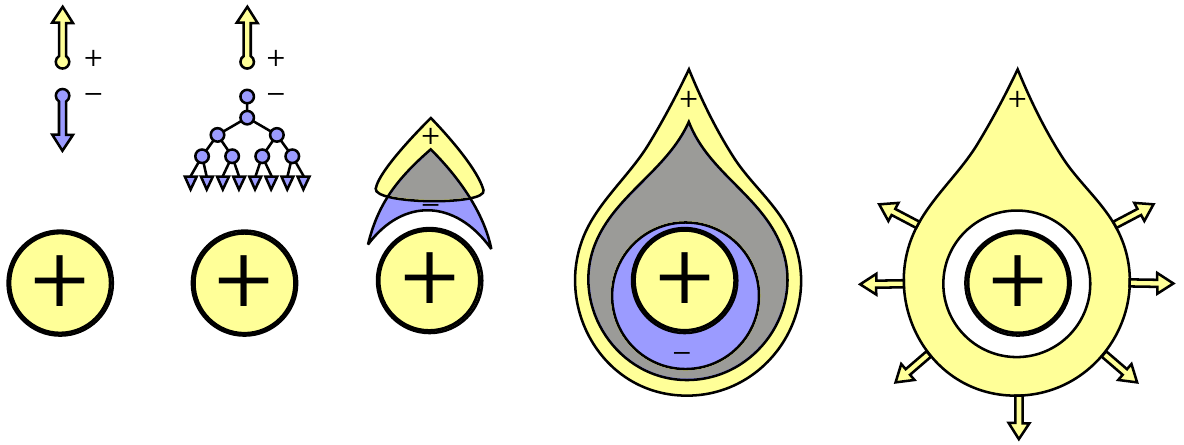
\includegraphics[width =0.7\textwidth]{figures/png/Screenshot_20240330_182509.png}
    \caption[The model of an ionisation avalanche forming at the anode wire of a proportional tube.]{The model 
    of an ionisation avalanche forming at the anode wire of a proportional tube or chamber \cite{kola}. 
    (a) In the drift volume, electrons and ions are generated and drift to their corresponding electrodes. 
    (b) Near the wire, the electron achieves a high enough field to induce secondary ionisation, resulting in an avalanche. 
    (c) The electric field separates charges created during an avalanche. 
    (d) Electrons have higher lateral diffusion than ions, causing the avalanche to expand 
    around the wire and produce a positive charge cloud in the shape of a drop. 
    (e) Electrons from the avalanche reach the anode within nanoseconds, but ions take longer, up to ms, to reach the cathode.}
    \label{fig:avalanche}
\end{figure}
\subsubsection{Avalanche Gain}
When an avalanche develops, the amplification factor is around $10^4-10^6$. The number of electrons freed per unit path length is given
by the first Townsend ionization coefficient $\alpha=\sigma_{ion}n=1/\lambda_{ion}$ and this depends on the electric field $E$, 
as a higher electric field corresponds to a higher kinetic energy of the electron, that increases the ionization cross-section.
The increase $dN$ of the number of electron-ion pairs over a path length $ds$ is \cite{kola}:
\begin{equation}
    dN=\alpha(E)Nds
\end{equation}
Solving this equation, we can easily obtain the gas amplification $G$:
\begin{equation}\label{av}
    G=\frac{N(s_a)}{N_0}=\text{exp} \left( \int_{s_0}^{s_a} \alpha(E(s)) ds \right)=\text{exp} \left( \int_{E_{min}}^{E(a)} \frac{\alpha(E(s))}{dE/ds} dE \right)
\end{equation}
where $N_0$ corresponds to unamplified electrons in $s=s_0$ and $E_{min}$ corresponds to the minimum energy 
for ionisation to occur. The energy distribution depends on the electric field which is position dependent. 
Since the free path is inversely proportional to the particle density in the gas, $E_{min}(\rho)=E_{min}(\rho_0)\rho/\rho_0$.
It is reasonable to say that the coefficient is proportional to the field strength, $\alpha= \beta E$, in the low field region. 
Adding this relation with Equation \ref{avalanche} and \ref{av}:
\begin{equation}
     \text{ln}(G)=\beta \ a \ E(a) \ \text{ln}\left( \frac{E(a)}{E_{min}}\right)
\end{equation}
where $\beta$ can be related to $w_i$, that is the energy spent for one ionisation and its value is equal to $e \Delta V$.
As the voltage drop per unit path length is $dV = E(s)ds = (\alpha/\beta)ds$, we obtain $dN=N \beta dV$. Integrating, we can see that
$\beta= \text{ln}(2)/\Delta V$, so the gain in a drift tube is:
\begin{equation}\label{XXX}
     \text{ln}(G)=\frac{ \text{ln}(2)}{\Delta V} \ a \ E(a)  \ \text{ln}\left( \frac{E(a)\rho_0}{E_{min}(\rho_0)\rho}\right) \qquad E(a)=\frac{V}{a \cdot \text{ln}(b/a)}
\end{equation}
which is the Diethorn's formula. 
Gain measurements with variable $\rho$/$\rho_0$, $a$, and $E(a)$ can provide the parameters $E_{min} (\rho_0)$ and $\Delta V$. 
The gas temperature $T$, pressure $P$ and operating voltage $V$ significantly impact
the gain of a drift tube and gas mixture. 
\subsubsection{Quench Gas}
To avoid subsequent avalanches, the drift tube gas combination may contain a quench gas, such as CO$_2$, 
methane, or other hydrocarbons. During an avalanche, photons are created by gas deexcitation and electron 
attachment to electronegative species, resulting in negative ions. Photons can generate ionisations 
outside the primary avalanche zone or create free electrons on the cathode surface, resulting in secondary avalanches.
The difficulty arises when the signal created is not proportional to the deposited energy by the original particle 
and is no longer localised to the energy deposition point. Enough intense photons can induce a chain reaction of 
secondary avalanches, leading to a continuous discharge. The use of quench gas prevents subsequent 
avalanches by absorbing ionising photons before they travel far. A tiny quantity of quench gas during normal operation 
can significantly decrease secondary avalanches and breakdowns.
\subsubsection{Operation Modes of Gaseous Ionization Detectors}
In drift tube detectors, the number of electron-ion pairs formed during an avalanche is 
proportional to the starting number of electrons, as shown in the gain computation. To 
operate in a proportional mode, an appropriate voltage is needed to reduce the effects 
of avalanche charges on the electric field. Figure \ref{fig:gaseous} illustrates how a 
gaseous ionisation detector may work in multiple modes based on the operating voltage. Higher operating 
voltage leads to higher charges on the electrodes. Low voltage power supply causes ionisation charges to recombine 
before reaching electrodes, leading to no signal collection. At higher voltages, in ionisation chamber 
region, charges can drift to electrodes, but the electric field is insufficient for avalanches to occur. 
Increasing the operational voltage leads to drift tubes and proportional counters. When the voltage 
becomes high enough, proportionality is lost. When electrons from an avalanche are collected, 
the high density of positive ions near the anode might affect the electric field. 
Electrons in future avalanches that enter the area between the positive ion cloud and the wire face a 
decreased electric field, resulting in lower amplification. The electric field becomes greater in the 
tail of the avalanche, which is far from the wire than the ion cloud. This range of voltage is called region of 
limited proportionality. When the operating voltage reaches high values, 
avalanches create sufficiently energy photons to cause secondary avalanches 
that propagate across the detector, independently from the quench gas. 
This results in detector saturating the output. This way of operating is 
called breakdown mode, commonly known as the Geiger-Muller mode.
\begin{figure}[!h]
    \centering
    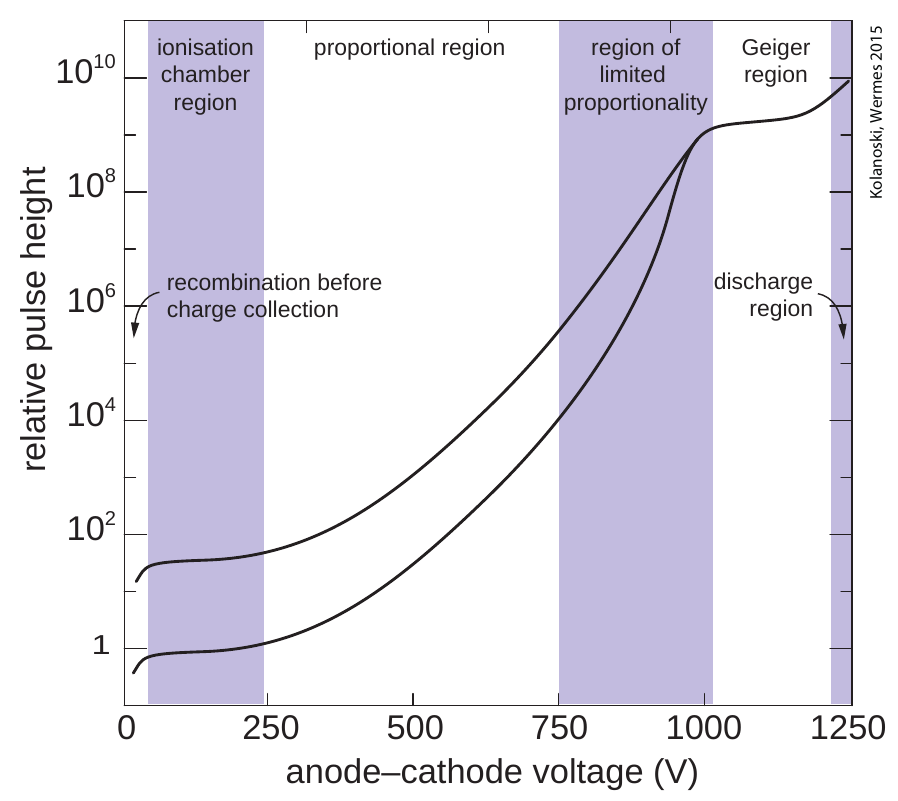
\includegraphics[width =0.5\textwidth]{figures/png/Screenshot_20240330_203416.png}
    \caption[The dependence of output signal of a counting tube 
    on the applied voltage in gaseous ionisation detectors.]
    {The dependence of output signal of a counting tube 
    on the applied voltage in gaseous ionisation detectors.  
      The numbers on the axes are for orders of magnitude only and they depend on the device geometry
      and gas concentration. 
    Drift tubes operate in the proportional mode \cite{kola}.}
    \label{fig:gaseous}
    \end{figure}
\subsection{Signal creation and propagation}
Drift tube signals do not come directly from avalanche charges. 
If they did, the anode wire would receive the entire signal 
in just a few ns. Instead, signals are generated due to the 
movement of charges on the electrodes, influenced by the 
mobility of electrons and ions. The Shockley-Ramo 
theorem \cite{kola}, can be 
used to determine the induced charge and current. 
One of the key results of this theorem is that 
the total induced charge of a moving charge 
is determined by the initial and final positions only.  
A charge pair induces the same amount of 
charge on an electrode as the charge collected on it. 
Furthermore, if all electrodes are treated as 
an unity, their weighted potential will be one. 
If one electrode completely encloses the others, the 
weighted field in the contained region is always zero. 
This means that the total induced current across all 
electrodes is always zero.
Applying this to the drift tube, the theorem 
helps us analyze the induced current signal produced by an 
avalanche of electron-ion pairs on the anode wire. 
When compared to the total charge induced $Q^{ind}_{tot}= -eN$, 
electron mobility in the avalanche accounts for just 1-2\%. 
Positive ion drift from the avalanche accounts for the majority of the signal. 
A signal propagates to both ends of the drift tube from the avalanche location.
Signals with distinct frequency components can propagate at varying velocities. This causes the signal to disperse. 
For more details, refer to \cite{kola}.
%For low-frequency components of the signal (for a meter-long drift tube, this translates to a frequency much less than 300 MHz), 
%a quasi-electrostatic approach is sufficient. The signals seen at tubes ends are influenced by impedances between and on the electrodes. 
%On the other hand, for the high-frequency components of the signal, the tube needs to be treated as a transmission line. 
%The propagation speed of a signal wave with frequency $\omega$ is then $c/\sqrt{\omega}$ $\epsilon$($\omega$), 
%where $c$ is the speed of light and $\epsilon$ is the dielectric constant of the gas. As $\epsilon$ is a function of $\omega$, 
%components of different frequencies propagate at slightly different velocities. This leads to a dispersion (widening) of the signal. It brings some subtleties when using signal arrival time difference between straw tube ends to determine the longitudinal coordinate of an avalanche.
\section{The Mu2e straw tracker}\label{geomtra}
The sensitive elements of the detector are straw-tubes with a diameter of 5 mm and a variable length between 40 cm and 110 cm, 
filled with a 80\%:20\% Ar:CO$_2$ mixture at 1 atm.  
The detector has a modular design, made of basic elements named $Panel$, $Face$, 
$Plane$ and $Station$, shown in Figure \ref{fig:trkpanel}. 
The panel is the fundamental unit of the detector: 96 straw tubes arranged like 
harp cords in two staggered layers to form one harp-shaped panel spanning 120° along the azimuthal angle \cite{bartoszek2015mu2e}, 
shown in Figure \ref{fig:trkpanel} (top left).
Three rotated panels form a face, and two faces rotated of 30° form one plane, Figure \ref{fig:trkpanel} (top right-left). 
Two planes are coupled to make a station, mounting the second rotated on the vertical axes by 180°.
Figure \ref{fig:trkpanel} (top right-right).
One station is thus made of twelve panels. The entire tracker is made of 18 stations, Figure \ref{fig:trkpanel} (bottom) 
and has a total length of 3.2 m and a diameter of approximately 1.7 m.
Each panel is equipped with its own Front-End and DAQ electronics placed within the mechanical structure (colored in red).
\begin{figure}[!h]
\centering
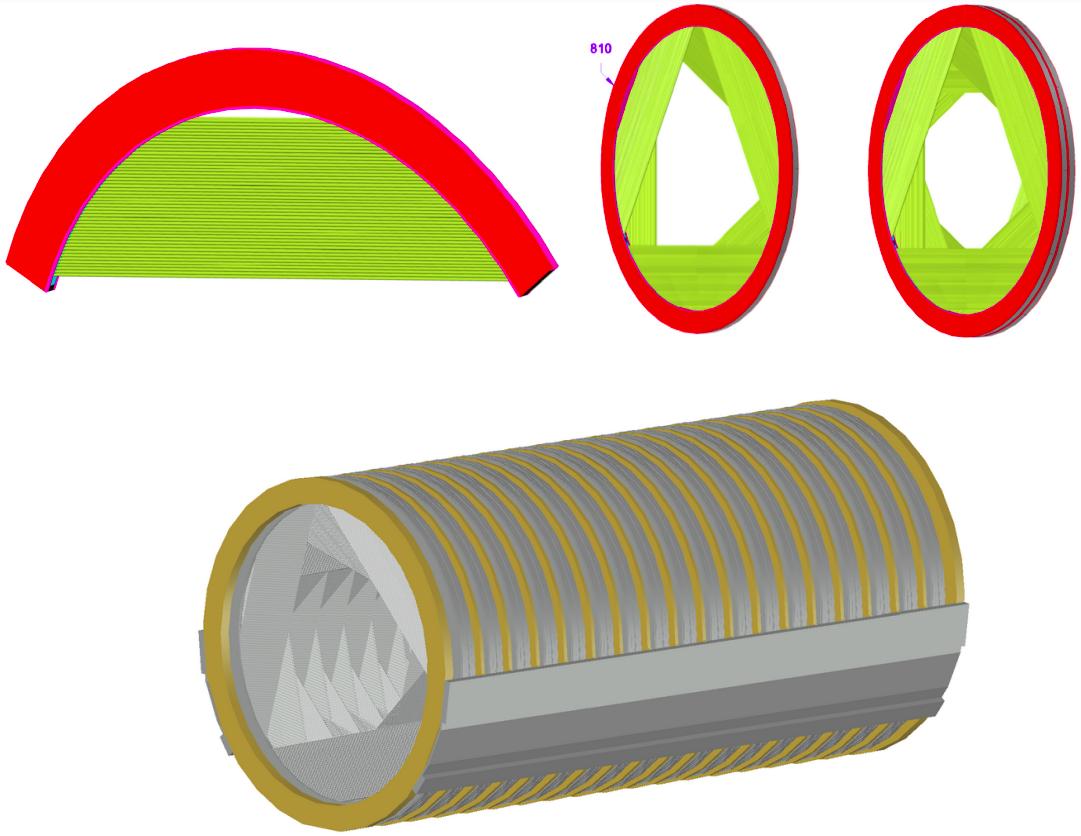
\includegraphics[width =0.6\textwidth]{figures/png/Screenshot_20240306_222803.png}
\caption[The straw tracker components.]{(Top left) Schematic representation of one straw tracker panel. (Top right) 
Straw tracker plane (left) and station (right). (Bottom) Full assembly of the 18 
stations and support structure \cite{bartoszek2015mu2e}.}
\label{fig:trkpanel}
\end{figure}
\subsection{The sensitive unit: the straw}

The Mu2e tracker straw tubes use the same detection principles as the gaseous 
ionisation detectors \cite{kola}, to 
meet the experiment precise requirements.
Figure \ref{fig:trkpencil} shows the edge of a straw tube, compared to a pencil.
\begin{figure}[!h]
    \centering
    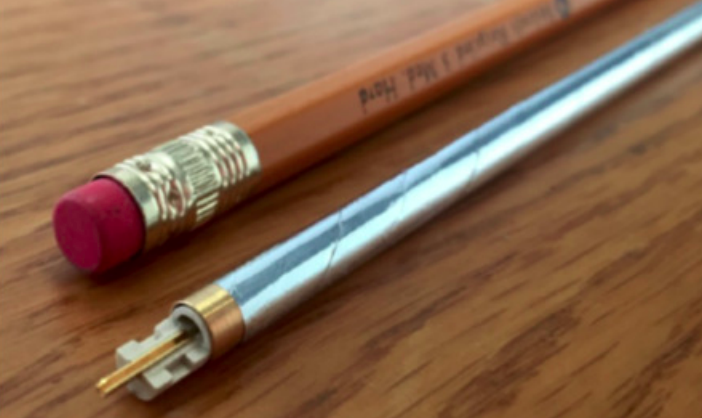
\includegraphics[width =0.5\textwidth]{figures/png/Screenshot_20240327_000000.png}
    \caption[A Mu2e straw tube.]{One of the Mu2e straw tube (compared to a pencil) \cite{trk}.}
    \label{fig:trkpencil}
    \end{figure}


All the straws have the same diameter of 5 mm, but their length 
is between a maximum of 334 mm and a minimum of 1.174 m, 
depending on their position on the panel, as shown in Figure \ref{fig:gonzalo}.

The straw is wound with two layers of 6 $\mu$m-thick metallized 
Mylar separated by one 3 $\mu$m layer of glue. The straw wall is thus 15 $\mu$m thick: 
this minimizes the amount of detector material and thus the total energy 
loss of electrons in the detector. Moreover, this minimises the probability 
of significant deflections of the electron trajectory which makes pattern 
recognition and track reconstruction much simpler both at trigger 
and offline level, and allows to achieve the required excellent momentum 
resolution. The straw tube anodes are made of gold-plated tungsten wires with 
a diameter of 25 $\mu$m. The straw and the anode wires are tensioned 
and work-hardened to minimise sagging effects.
Figure \ref{fig:trktubessmon} shows the straw termination machanical 
structure that allows to hold the anode wire in place.
To increase the straw mechanical strength, two brass tubes 
are joined to both ends of the straw suing silver epoxied.
    \begin{figure}[!h]
        \centering
        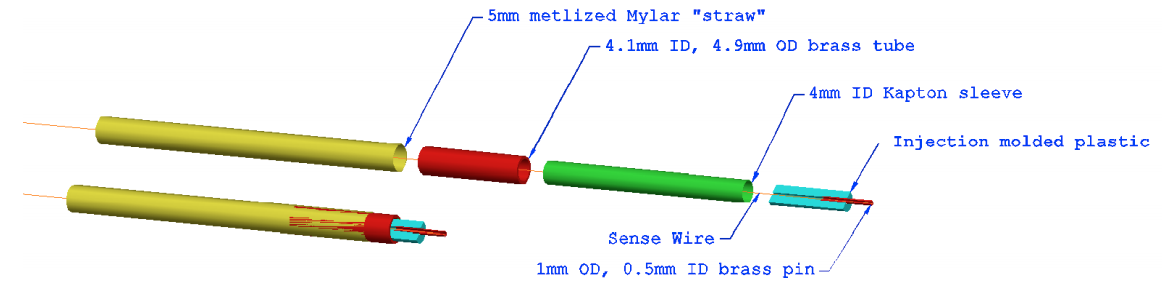
\includegraphics[width =\textwidth]{figures/png/Screenshot_20240706_153158.png}
        \caption[The straw termination.]{The straw termination, depicted both exploded and assembled, 
        features a brass tube connected to the straw using silver epoxy. 
        An insulator (green) is inserted into a brass tube 
        (red) to prevent breakdown near the tube's end. The sense 
        wire is soldered into the brass pin and epoxied to the 
        injection-molded plastic. Post-assembly, the brass tube 
        facilitates connection to the cathode, while the brass pin 
        enables connection to the anode.}
        \label{fig:trktubessmon}
        \end{figure}
        To ensure electrical insulation of the anode wire, 
        a kapton sleeve is inserted inside the brass tube. 
        The kapton sleeve holds an injection-molded plastic 
        insert which cointains a semicylindrical duct that 
        allows gas flow into and out of the tube. The insert 
        has a groove along its axis and a U-shaped brass anode 
        pin inserted at the end. To avoid slippage, the anode 
        wire is epoxied into the groove and soldered to the 
        anode pin. A T-shaped pin protects the anode pin from 
        breaking by covering the groove in the plastic insert. 
        The pin protector is epoxied to the insert with an extra 
        brass ring connecting them. A ground clip is silver-epoxied 
        to two adjacent straws on the brass tubes and rings to 
        provide a shared ground connection.
        To optimise the shape of the electric field within 
        the straw, assembly procedures have been developed 
        to align the anode wires to the panels with a 
        precision of at least 25 $\mu$m in the radial direction and 50 $\mu$m in the perpendicular direction. 
From the straws, signals are sent to a common preamp board 
via the anode pin pair and grounding clip. The tracker front 
end eletronic will be described in Section \ref{tfee}.
\subsection{The building blocks: from the panels to the station}
Groups of 96 straws are assembled in two staggered layers of 48 straws and make a 
panel (Figure \ref{fig:trktubes}). 
\begin{figure}[!h]
\begin{subfigure}[t]{0.5\textwidth}
    \centering
    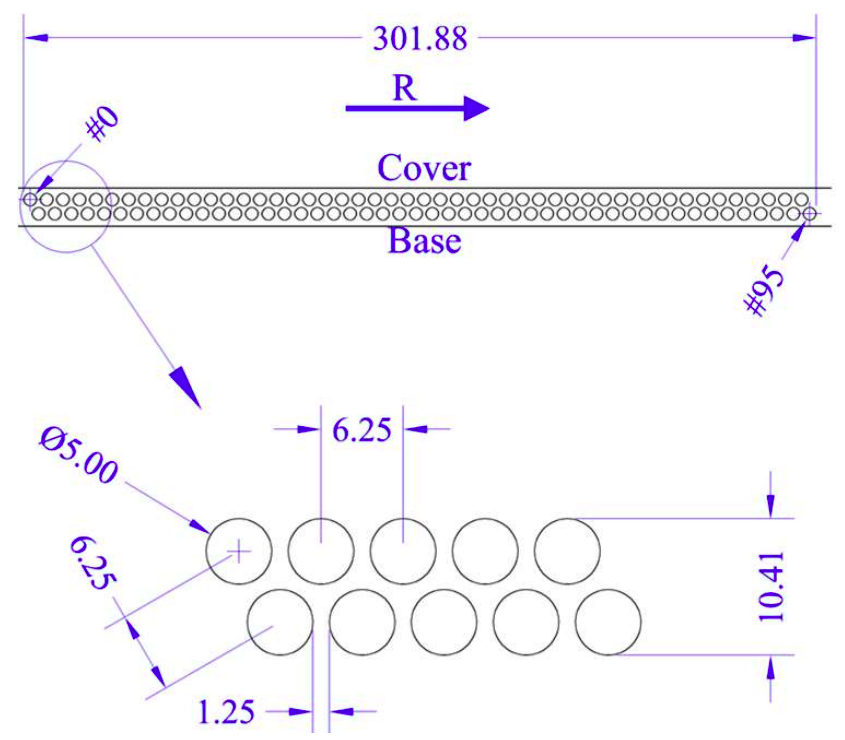
\includegraphics[width =\textwidth]{figures/png/Screenshot_20240326_234405.png}
    \caption{}
    \label{fig:trktubes}
    \end{subfigure}
    ~
    \begin{subfigure}[t]{0.5\textwidth}
        \centering
        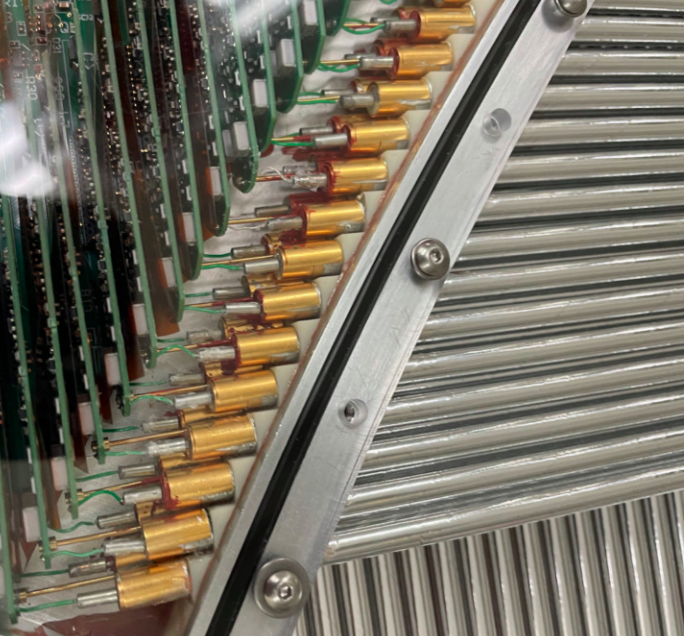
\includegraphics[width =\textwidth]{figures/png/Screenshot_20240327_000131.png}
        \caption{}
        \label{fig:strawtubes}
        \end{subfigure}
        \caption[The straw arrangement within a panel.]{(a): The straw arrangement within a panel \cite{trk}. (b): Expanded view of the panel edge \cite{trk}.}
    \end{figure}

Each panel spans a 120° arc (Figure \ref{fig:gonzalo}).
The dual-layer geometry was chosen to maximize the total panel coverage. 
This simplifies pattern recognition and increases tracking robustness and efficiency. 
A 1.25 mm separation between two consecutive straws accommodates 
manufacturing tolerances and allows for straws expansion due to gas 
pressure. This requires each straw to be self-supporting across its 
length. Channels within a panel are numbered from 0, 
corresponding to the radially most internal and longest straw, 
to 95, corresponding to the most external and shortest straw. 
An expanded view 
of the panel edge is shown in Figure \ref{fig:strawtubes}.
            \begin{figure}[!h]
                \centering
                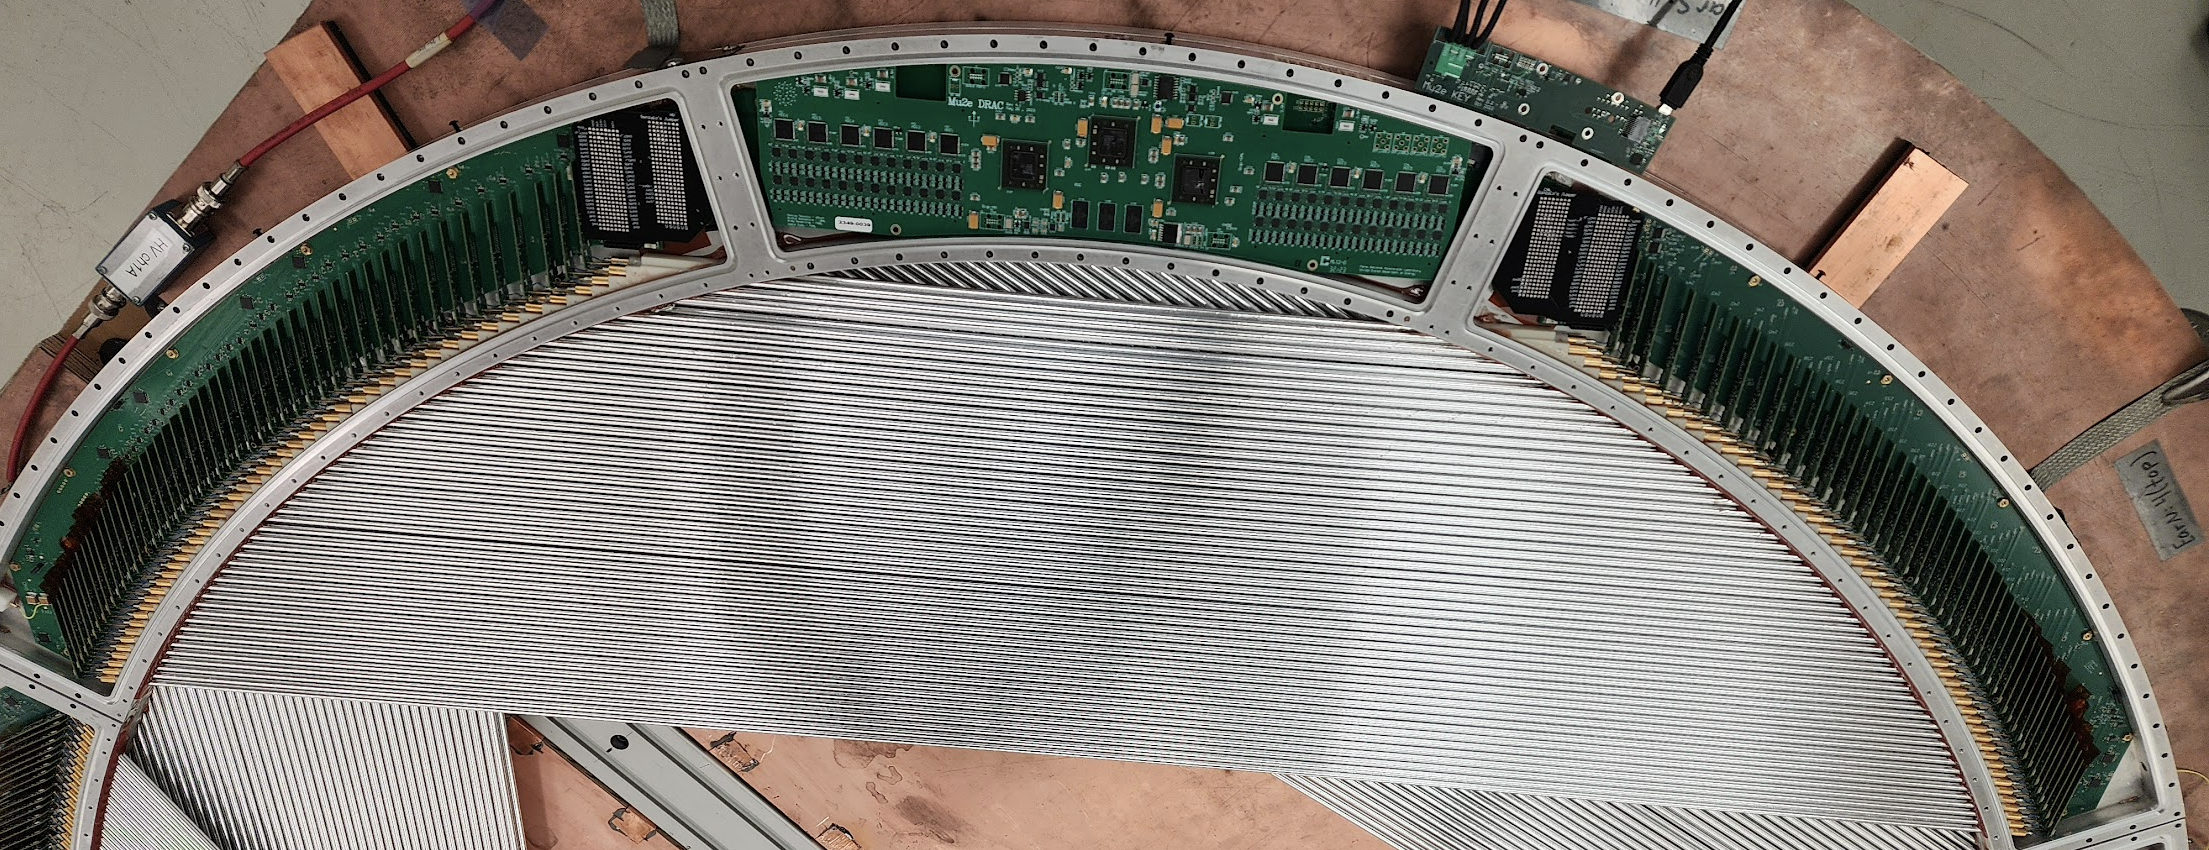
\includegraphics[width =\textwidth]{figures/png/image.png}
                \caption[One of the fully assembled panel.]{One of the fully assembled panel (Lab3 Fermilab Facility).}
                \label{fig:gonzalo}
                \end{figure}

            The straws are filled with a gas mixture of 80\%:20\% Ar:CO$_2$ at 1 atm.
            Since the DS internal volume is evacuated to 10$^{-4}$ Torr, 
            the straws must endure such pressure difference. Under normal temperature and 
            pressure conditions, the panel must have an average leak rate below 0.014 cm$^3$/min.  
            The nominal operating voltage of the straw is 1450 V. 
            Preliminary tests showed that the straw 
            tube gain is 1.25 $\times$10$^4$ at 1250 V and 7 $\times$ 10$^4$ at 
            1425 V. According to Diethorn's calculation, Equation \ref{XXX}, 
            the gas gain at 1450 V is around 1 $\times$10$^5$.
 

All panels are x-ray scanned 
to accurately measure and document the wire 
locations of straw tube channels. 

Three panels rotated of 120° make a face and two faces rotated of 
30° make a plane (Figure \ref{fig:trkpanel} (Upper right-left) and \ref{fig:trueplane}).

Once a plane is assembled, a cooling ring is fitted around its outer circumference. 
The Front-End electronics is hosted in a ring around the outer 
circumference of the panel.

Two identical planes rotated of 180° around a vertical axis make one station 
(Figure \ref{fig:trkpanel} (Upper right-right)). 
During assembly, the second plane is rotated of 180° around the vertical axis.

At the moment of writing this Thesis, almost all tracker planes have 
already been assembled at Fermilab Lab3 Facility and the station assembly was in progress, 
as shown in Figure \ref{fig:trueplane}.

\begin{figure}[!h]
    \centering
    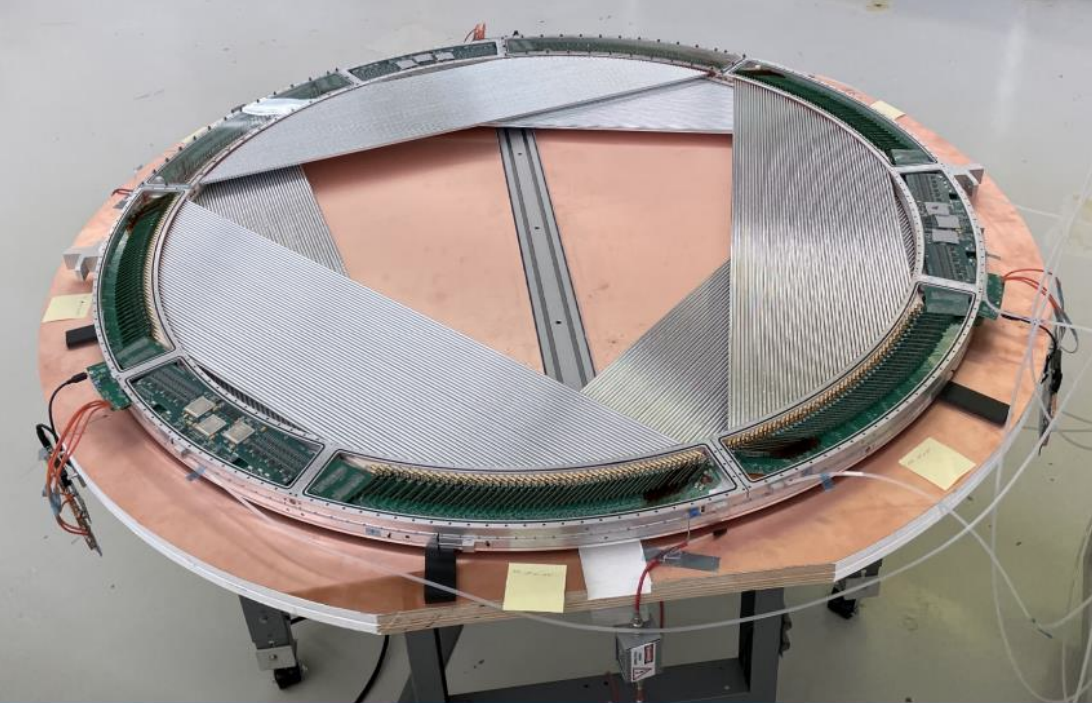
\includegraphics[width =0.65\textwidth]{figures/png/Screenshot_20240706_163056.png}
    \caption[One tracker plane fully assembled.]{One tracker plane fully assembled at Fermilab Lab3 Facility.}
    \label{fig:trueplane}
\end{figure}
\subsection{The entire straw tracker detector}

The entire detector is made of 18 stations (Figure \ref{fig:trkpanel} 
(bottom)) assembled together with a complex mechanical structure. 
Horizontal beams maintain longitudinal alignment of the rings. 
A thicker ring and two thinner rings placed at the downstream end 
of the detector stiffen the structure. The beams and the stiffening rings 
are made of stainless steel.

The detector rests on four bearing blocks attached to the 
stiffening rings and placed near the horizontal beams.
The connection between the detector and the bearing blocks 
is kinetic, to avoid over-constraining and distorting the frame. 
The only constraint of the four points is along the vertical 
direction, and vertical adjustment screws allow to level and 
center the frame. Once fully assembled, a thorough mechanical 
survey of the detector will be performed before moving to the Mu2e experimental hall. 

\subsection{The tracker Front-End Electronics}\label{tfee}
The Front-End electronics performs amplification, digitization and data packaging 
for transmission to the Data Acquisition System (DAQ) of the straw-tube signals. 
In particular, each single straw provides two hit times and one waveform, 
which are necessary to reconstruct the hit position along the straw, 
thereby allowing the use of constant fraction discrimination and mitigating time walk effects. 
A schematic representation of the entire system logic is reported in Figure \ref{fig:flowfee}.
\begin{figure}[!h]
    \centering
    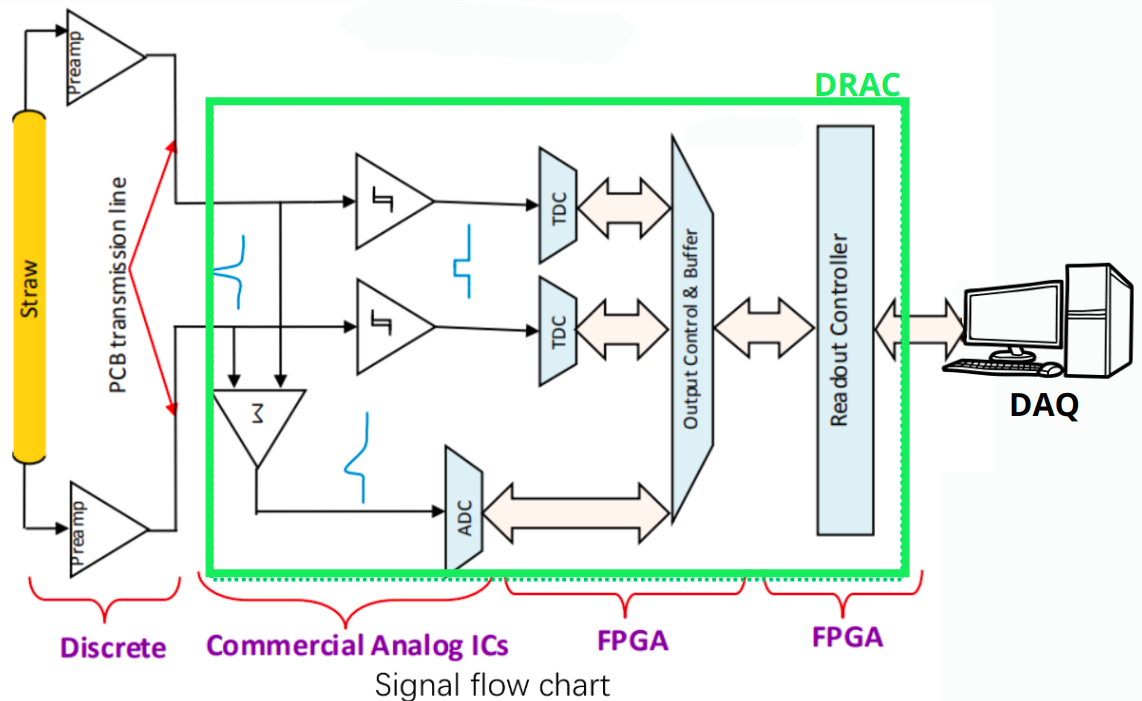
\includegraphics[width =0.9\textwidth]{figures/png/Screenshot_20240529_133230.png}
    \caption[Signal flow through Front-End electronics.]{Signal flow through Front-End electronics \cite{bartoszek2015mu2e}.}
    \label{fig:flowfee}
    \end{figure}
All the Front-End electronics is installed on multiple Printed Circuit Boards 
(PCBs) mounted on the outer section of the panel. 
The PCBs are shown in Figure \ref{fig:trackerfee} \cite{vadimmu2e}.
All PCBs are situated in the outer section of the panel. 
The panel has two sides, the high-voltage side (HV-side), 
which handles the high-voltage supply distribution to the straws, and 
the calibration-side (CAL-side), that contains the circuitry
to inject the calibration pulses.

Signals from the straw tube channels are first read 
out from both ends by the pre-amplifiers (preamps).

Both sides of the panel have one Analog Mother Board (AMB) and one Jumper board, 
whose task consist of directing signals from the preamps towards the Digital 
Motherboard (DMB) positioned at the center, then to the Digitizer Readout and 
Assembler Controller (DRAC) (mounted on top of the DMB) to be processed and 
temporarily stored. 

The AMBs and the DMB also handle 
low voltage distribution and the AMB on the HV side distributes the high voltage to the wires. 
The low voltage power supply is connected to the panel through the KEY board which 
contains also an optical fiber link and a JTAG connector. The AMB on 
the CAL side can inject a calibration pulse into the wires. 
The boards are also equipped with sensors to monitor environmental parameters, 
including temperature, pressure and humidity.

In addition, the frontends components were chosen to sustain high level of radiation.

The first step of signal processing is the signal pre-amplification performed 
by preamps mounted on two AMBs placed on the two lateral sides of the panel. 
The analog signals are transmitted from the preamps via 
microstrip transmissione lines and through a Jumper board to the DRAC.
Most of the data processing functions are performed by the DRAC board. 
The analog signals are processed by the Time-to-Digital Converters 
(TDCs) and by the Analog-to-Digital Converters 
(ADCs) installed on the DRAC. Digitized data are then transferred to the Readout 
Controller (ROC) for data packaging and transmission to the Mu2e DAQ 
(Figure \ref{fig:flowfee}). 

To summarise, each straw-tube is an independent detector channel equipped with:
\begin{itemize}
    \item two preamp channels, one for each end;
    \item two TDC channels, one for each end (192 in total);
    \item one ADC channel, measuring sum of both ends (96 in total);
    \item one High Voltage feed.
\end{itemize}
\begin{figure}[!h]
\centering
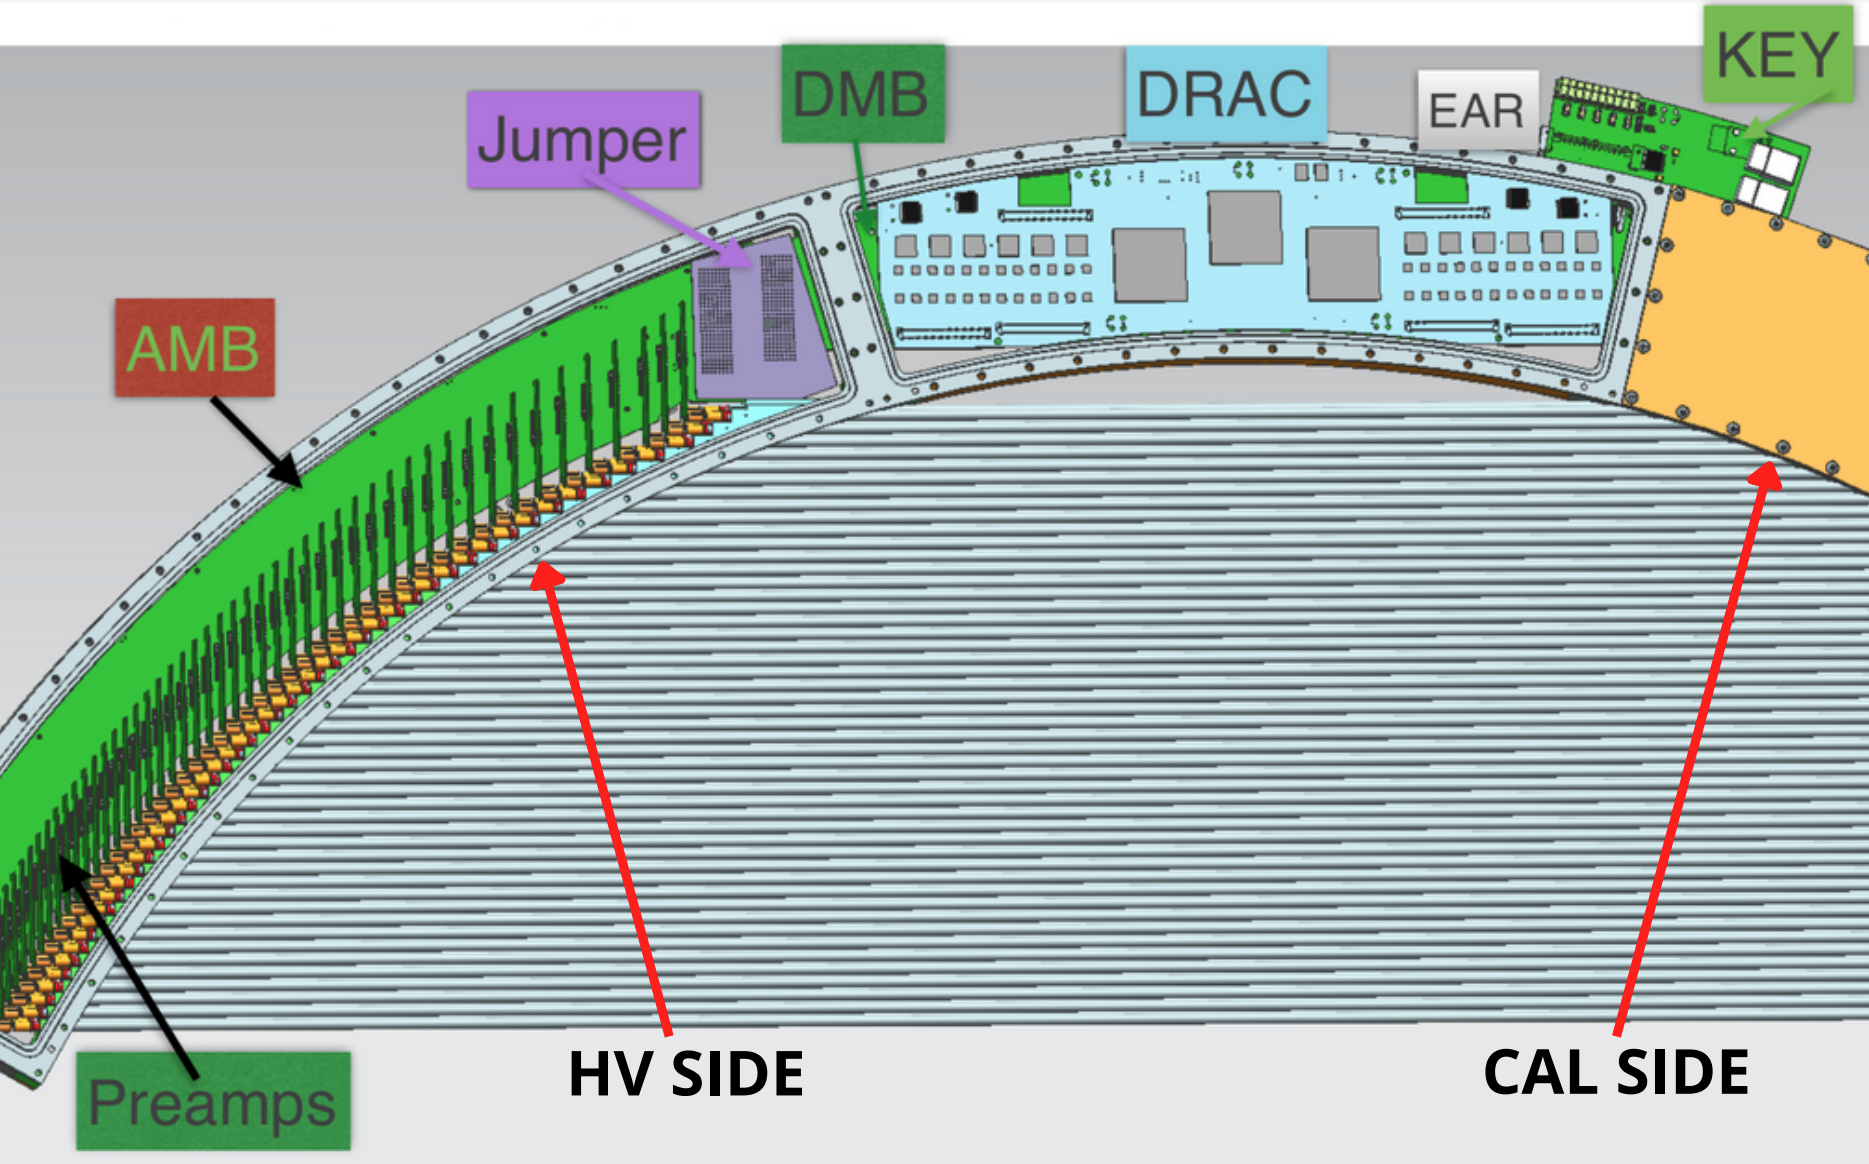
\includegraphics[width =0.8\textwidth]{figures/png/Screenshot_20240131_111836.png}
\caption[Overview of the straw-tracker Front-End electronics.]{Overview of the straw-tracker Front-End electronics  
\cite{vadimmu2e}. The CAL-Side of the panel is not shown.}
\label{fig:trackerfee}
\end{figure}


\subsubsection{The preamps}\label{preampss}
All the 96 straw-tubes are read out from both ends. 
Two adjacent tubes are connected to the same preamp PCB board. 
These boards are mounted vertically on the AMBs. 
Thus, each preamp PCB board contains two preamps,  
each one connected to one single straw end. 
Each panel is thus equipped with 48 preamp PCB boards on the HV 
side and 48 on the CAL side, 192 preamps in total.
To minimise signal reflections, the preamps have a matching 300 $\Omega$ input impedance. 
The function of the preamps is to convert the straw tubes 
current signals into voltage signals which are amplified and shaped. 

%The voltage gains of individual channels, different from the gas gain, are set by control signal from the DRAC. A bias voltage, adjustable for each side of a channel, is applied to the signals. 
\subsubsection{The Digitizer Readout and Assembler Controller board}\label{DRAC}
The $brain$ of the panel is called Digitizer Readout and Assembler Controller (DRAC) board. 
The DRAC performs digitization, packaging, temporary storage and data transfer to 
the Mu2e DAQ system. It also controls all the panel operations. The schematics of the 
Figure \ref{fig:drac} shows a picture of the board: comparators 
and ADCs, three DDR3 memory chips and three Field-Programmable Gate Arrays (FPGAs) 
are clearly visible. 
The two FPGAs on the left and on the right are named digi-FPGAs: 
each of them receives the data from 48 straw channels, performs data 
monitoring, buffering and assembles data packets which are then 
transferred to the central FPGA named Readout Controller (ROC) \ref{DRAC}. 
The ROC handles communication, monitors slow control variables and 
controls all panel operations.

\begin{figure}[!h]
\centering
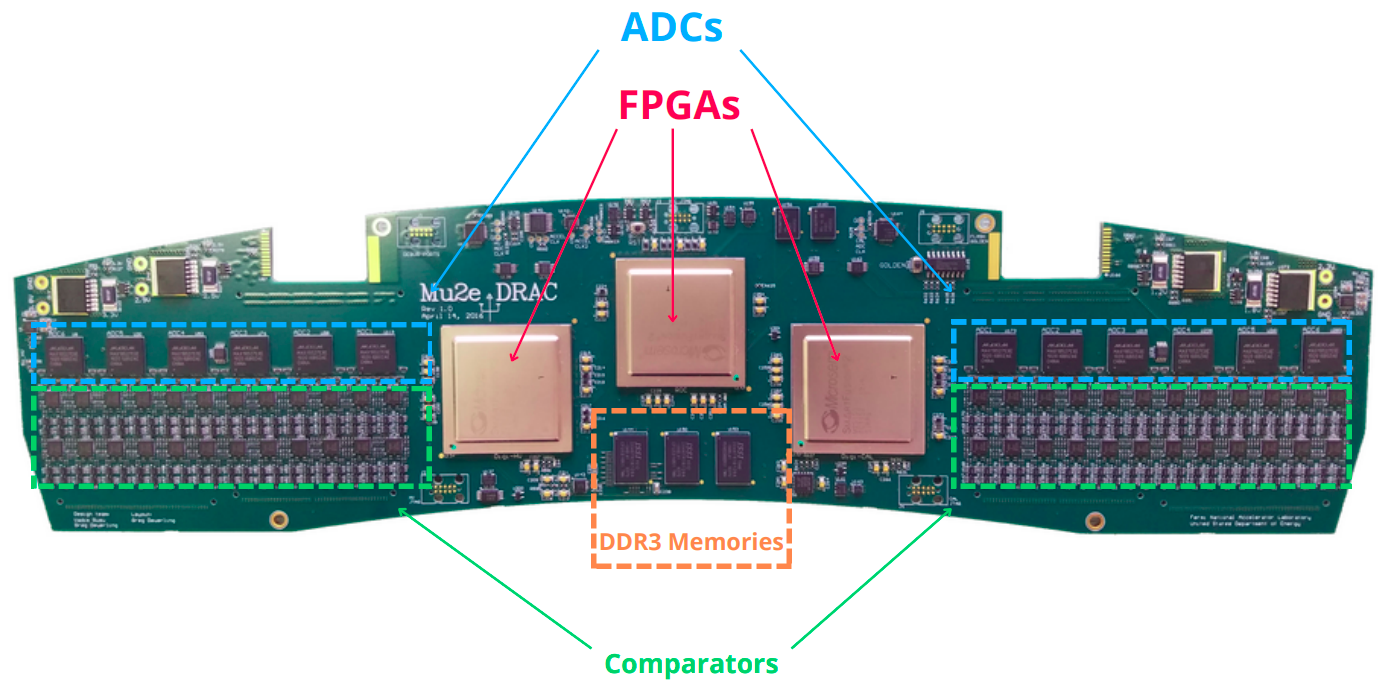
\includegraphics[width =\textwidth]{figures/png/Screenshot_20240204_115052.png}
\caption[The DRAC board schematics.]{DRAC board schematics \cite{drac}. 
The DRAC board is the brain of the tracker panel. ADCs, FPGAs, DDR3 
memories and compators are also shown.}
\label{fig:drac}
\end{figure}
Figure \ref{fig:flowfee} shows the data flow through the panel Front-End and the DRAC:
\begin{itemize}
    \item The two signals from the two sides of a straw tube are transmitted 
    from the preamps to the DRAC;
    \item In the DRAC, the two biased signals are fed to zero-crossing comparators, 
      which generate square signals if the signals are above their respective thresholds;
    \item The squared signals are transmitted to 16-bit TDCs implemented 
    in the firmware in the digi-FPGAs. Timing digitization bin is 20 ps, including the determination of the arrival time and the 
    time over threshold. 

  With the intrinsic TDC resolution of 25 ps, taking into account also the comparator jitter, 
    the noise and other external effects, the resulting time resolution 
    is of the order of 70 ps. At run time, a hit on a straw 
    is considered only if both ends of the same straw simultaneously have a 
    signal above threshold;
  \item Signals from the two ends of the same straw
    are also summed up, the sum is digitized by a 10-bit 
    ADC at 40 MHz and transmitted to the digi-FPGA;
    \item The digi-FPGA creates one data packet for each hit containing the 
    TDC and ADC information;
    \item The data packets are transferred to the ROC \ref{DRAC}, and 
    temporarily stored in the DDR3 memory for later access by the DAQ system. 
    There is a total of 8 Gb of memory space available on each DRAC. 
    The main function of the ROC is to collect data from the digitizer boards 
    digi-FPGAs, buffer data and transfer them to DAQ. ROCs continuously stream out 
    the zero-suppressed data collected between two proton pulses to 
    the Data Transfer Controllers (DTCs) (Section \ref{tdaqtra}) \cite{GIOIOSA2023167732}.
 The buffer stage is fundamental, since the DAQ is not able to handle the instantaneous 
 on-spill data rate and the off-spill time will be used to level the rate.
    The communication is flexible, thanks to the 
    programmable nature of digitizer, ROC and DAQ.
\end{itemize}

\subsubsection{The tracker data format}
Each event (hit) is composed of a data packet having a fixed length of 256 bits (32 bytes).
The packet has the following structure:
\begin{itemize}
    \item 16 bit header: the header contains information to uniquely specify this is a
    packet header, a channel identifier to specify the channel so the ROC can
    assign the hit to a wire number (straw index);
    \item 16 bit for the TDC left straw end;
    \item 16 bit for the TDC right straw end;
    \item The ToT (time-over-threshold) values for the two ends 
    of the straw are each stored using 8 bits;
    \item The ADC samples require 12 bits each. For each hit, a fixed number of 
    samples (15) is read out so we
    pack the samples tightly in order to fit the payload into two data per hit;
    \item 12 bits are set aside for preprocessing flags.
\end{itemize}

\subsubsection{The Data Acquisition System}\label{tdaqtra}

The Mu2e Data Acquisition system (DAQ) is based on a $streaming$ readout architecture: 
all detector data are digitised, zero-suppressed in the 
Front-End electronics 
and then transferred from the detectors for further 
processing and storage. 
This architecture results in a large data throughput in 
the DAQ but offers a 
significant flexibility for data selection and analysis. 
Figure \ref{fig:linktodaq}\cite{GIOIOSA2023167732}, 
shows the global 
architecture of the Mu2e DAQ. 
The Readout Controllers of all detectors are shown 
on the left side. The central box includes the main DAQ 
components: the Run Control Host, 40 DAQ servers, the 
Detector Control System (DCS), and the Event Building 
Switch. The Mu2e data rates will be substantial: for 
efficient data handling this segment of the DAQ heavily 
relies on firmware implementation. The right box includes 
the offline components, which perform data storage and 
offline processing. DAQ operation during data taking will be coordinated by the Run Control Host, 
which will manage a predefined Run Plan. During an active spill (approximately the first 
43 ms in the 48 ms bunch extraction cycle described in Chapter \ref{mu2echapter}), 
the experiment receives RF Zero-Crossing Markers from the Accelerator 
synchronised to the 1695 ns proton pulse cycles. This defines the 
Event Window\footnote{Event Windows are also assigned during off-spill periods 
when no beam batches are received. 
These Event Windows are longer due to the reduced data rate.}. 
Based on these markers, the Command Fan-Out (CFO) module 
generates a 40 MHz system clock and embeds Event 
Window Markers (EWMs) into this clock to denote the start of event 
windows. The CFO distributes this encoded system clock and run control 
packets to the DTCs in the DAQ servers. 
DTCs then pass the encoded clock to the ROCs within the detectors, 
where the EWMs are recovered with a fixed latency relative to the 
initial RF Zero-Crossing Markers. The local ROCs use the EWMs to distinguish 
data collected during consecutive Event Windows. For the tracker, 
this involves generating a DDR3 memory address at the start of each 
Event Window to store tracker hits recorded during that period. 
Data readouts from the ROCs to the DAQ system are triggered by Data Requests. 
The Data Requests can be configured via the CFO as per the Run Plan and are 
typically issued to the tracker and calorimeter ROCs following each event 
window through the DTCs. Conversely, the CRV Data Requests are issued via 
software. The ROCs respond to these Data Requests by transmitting the 
corresponding data to the DTCs. Data from multiple DTC sources are routed 
through the Event Building Switch to a designated DTC, pre-processed, and 
then transmitted to the Online Processing module within the same DAQ 
server\footnote{The DTCs are implemented as commercial PCIe cards located 
within the DAQ Servers.}. If a trigger decision is made, the corresponding 
CRV data are also read out from the ROCs through software-generated Data 
Requests. Event data from all detectors are collected at the Data Logger 
and transferred to the long-term storage. Calculations estimate a data rate of 35 GBps 
from the ROCs and an annual storage requirement for the entire experiment of 
approximately 7 PB. 

In addition to the detector data, the DTCs also handle the acquisition of 
slow control variables from the detectors. For the tracker, these variables 
include panels temperature, pressure, humidity, voltages, and currents at 
specified PCB boards, high voltages, and channel threshold settings across 
all panels. These data are managed by the DCS Host and recorded in long-term 
storage. The data are also accessible in real-time in the Control Room for 
monitoring purposes. Other detector control tasks and operations are managed 
through DCS commands via the DTCs. For the tracker, this includes panel 
configuration, calibration using preamp-generated pulses, and disconnection 
of channel high voltage when necessary. 

\begin{figure}[!h]
    \centering
    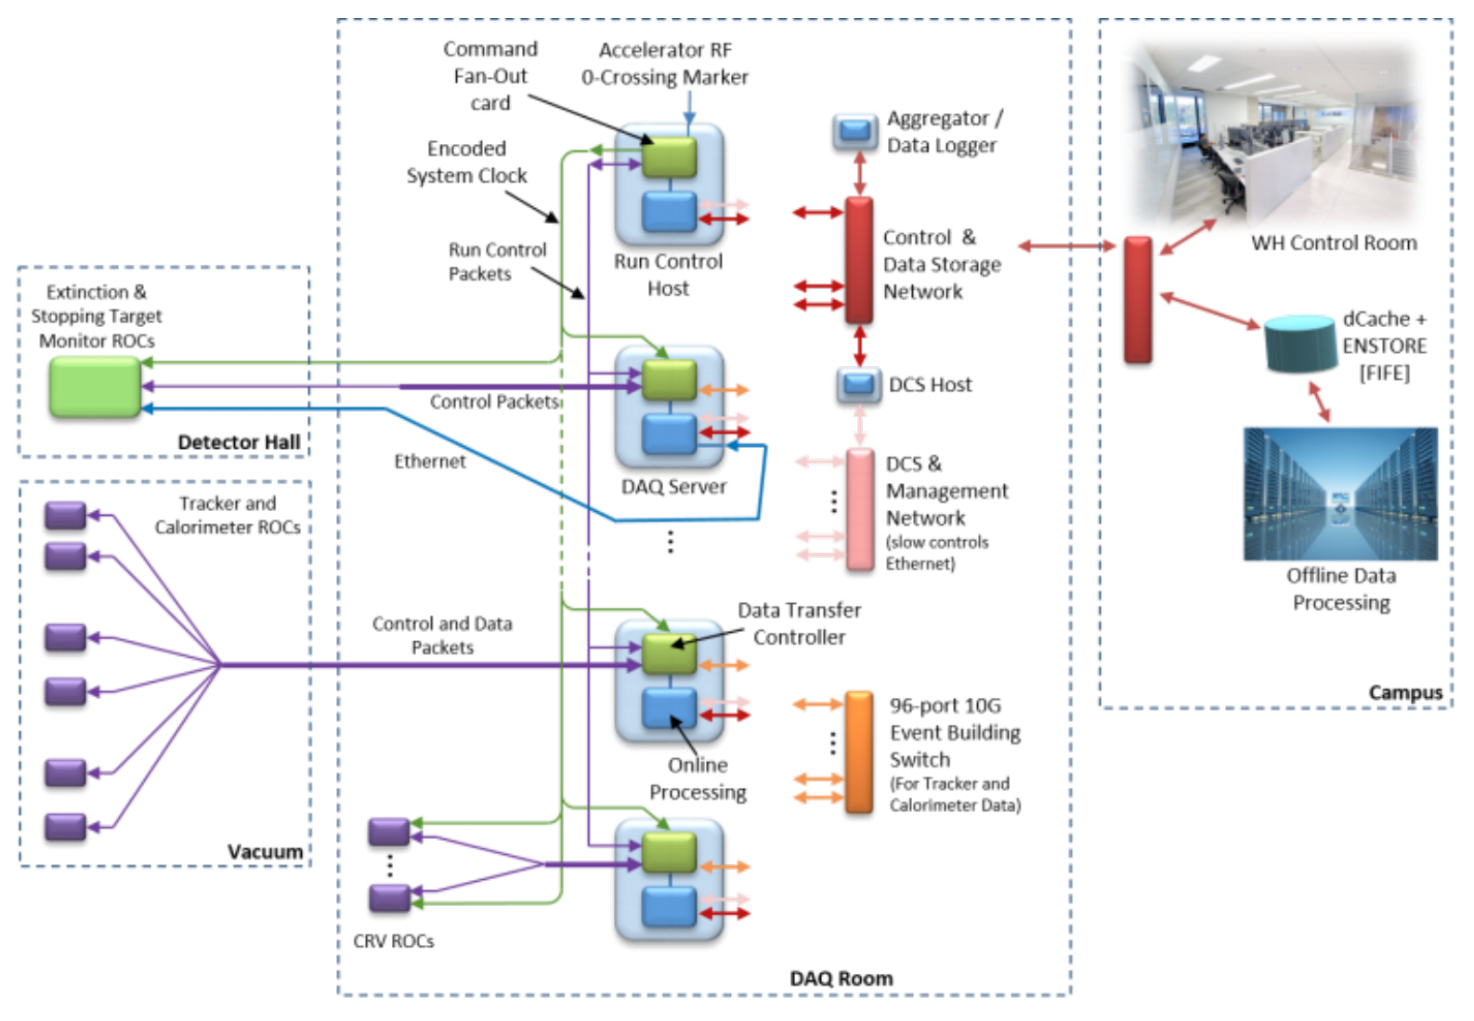
\includegraphics[width =0.8\textwidth]{figures/png/Screenshot_20240206_144803.png}
    \caption[The Mu2e Data Acquisition system architecture.]{Mu2e Data Acquisition system architecture \cite{GIOIOSA2023167732}.}
    \label{fig:linktodaq}
    \end{figure}



\subsection{Tracker performance requirements}
Here a resume of the requirements that the tracker must satisfy to ensure the 
success of the experiment is presented \cite{trkreq}.
A momentum resolution less than 180 keV/c for a 105 MeV/c electron is needed in the nominal
1 T solenoidal field, as measured at the front face of the tracker volume (before
passing through any tracker related material). Non-Gaussian tails, particularly any
high-side tail, must be controlled such that the DIO background results in much less
than one event at design sensitivity. To reach this, simulation results indicate that 
a single straw requires around 4 cm of longitudinal and 200 $\mu$m of transverse 
resolution for drift path lengths. 
It must have an acceptance of approximately 20\% for conversion electrons.
The tracker must operate in an ambient vacuum (< $10^{-4}$ Torr) and be able to withstand a rate of 5 MHz per straw (highest rate straw) 
500 ns after the spill. 
